%\documentclass[danish, a4paper, twocolumn, oneside]{memoir}
%\usepackage{A1_preamble}
\documentclass[A2_main.tex]{subfiles}

\begin{document}
\section{Databehandling}
\subsection{Grundfrekvensens afhængighed af snorspænding}
Vi har lavet to målinger hvor vi primært har kigget på \cref{eq: swave} og vi har derfor foretaget varibel kontrol og altså varieret på $\mu$ og $F$ i \cref{eq: wave}. Observationerne kan ses i \cref{fig:frekvensSNor}.
\begin{figure}[H]
    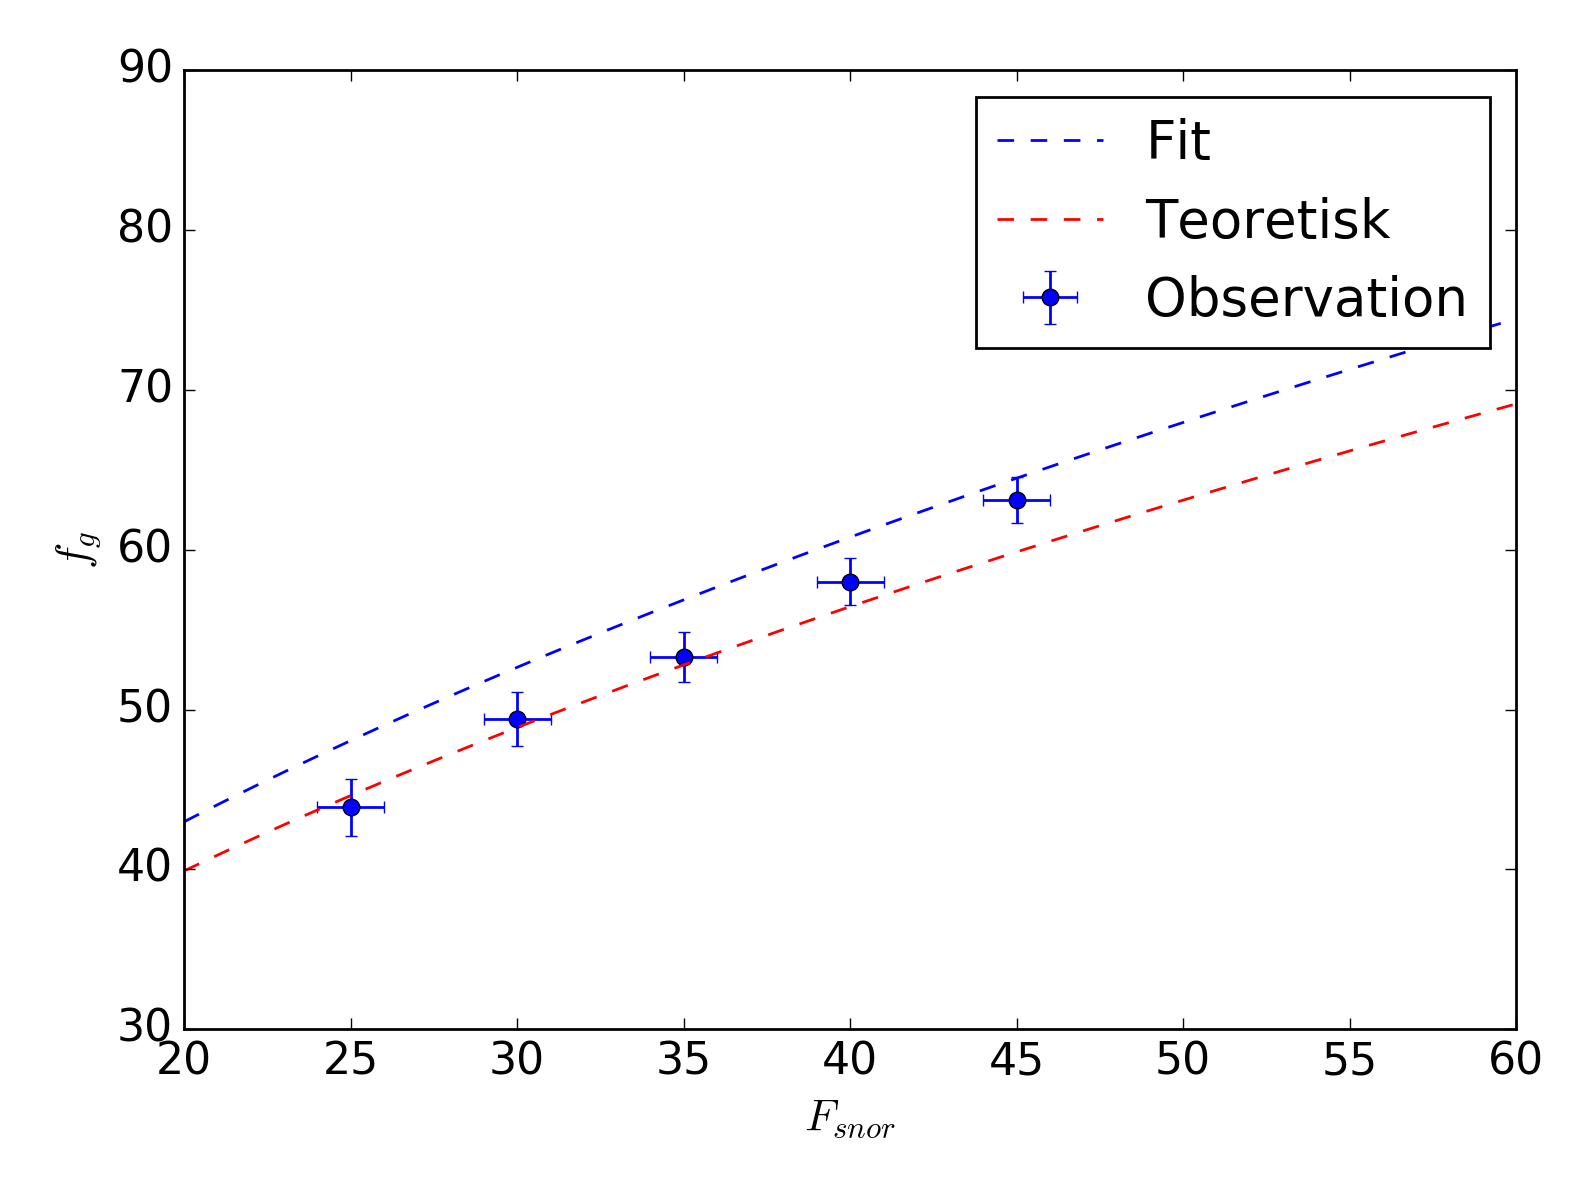
\includegraphics[width=\linewidth]{frekvensSnorSpaending.png}
    \caption{Resultater af fit, teoretisk værdier og observation af grundfekvensen som funktion af snorspændingen.}
    \label{fig:frekvensSNor}
\end{figure}

Her ses det at vi har lavet en fittet linje sammen med den teoretiske. Dette var for at se hvor godt et evt. fit ville være ift. teorien og ud fra dette fit har vi fundet en eksperimentielt bestemt værdi for $\mu$. Den er fundet til $\mu_{eks}=\SI{7.52e-3}{\kg\per\m}$. Den egentlige værdi for $\mu=\SI{8.72e-3}{\kg\per\m}$. Dette er rimelig tæt på den værdi vi fandt, men der er alligevel en rimelig afvigelse. Det skyldes sandsynligvis den outlier som vi har på vores data, som man måske skulle se bort fra - dette har vi valgt ikke at gøre grundet det lave antal målinger i forvejen. Det kan også lige nævnes at vores usikkerheder her er en rimelig faktor som det fremgår i \cref{fig:frekvensSNor}.
\subsection{Grundfrekvensens afhængighed af masse/længde}
Igen foretages varibel kontrol af samme \cref{eq: wave} Hvor snorspændingen $F$ og længden $L$ holdes konstant.
\begin{figure}[H]
    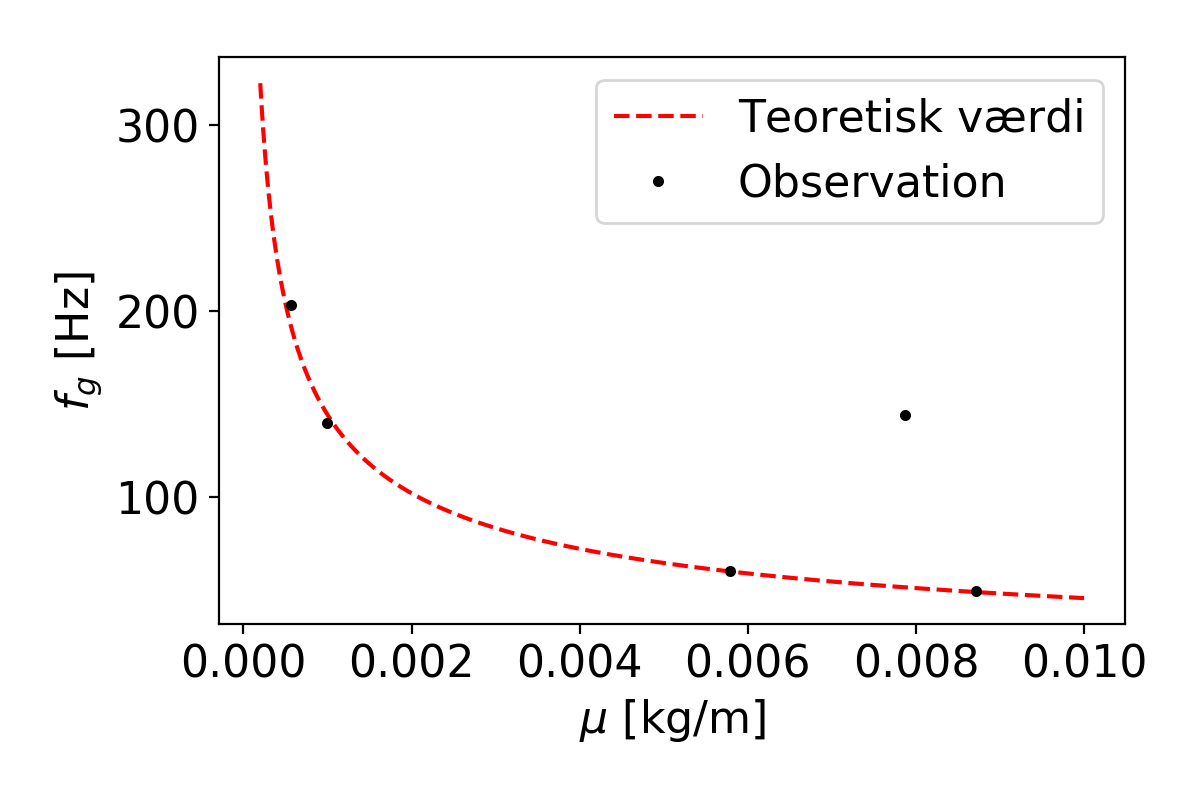
\includegraphics[width=\linewidth]{frekvensMu.png}
    \caption{Resultater af observationer og teoretiske værdier, af grundfrekvensen som funktion af snorspændingen.}
    \label{fig:frekvensMu}
\end{figure}
Her ses det at data passer rigtig godt på vores målepunkter, undtagen den ene outlier. Usikkerhederne her er ikke synlige grundet de store dimensioner på vores akser, men det kan nævnes at de er i omegnen af $\SI{\pm 5}{\Hz}$

\end{document}
